\section{Observability Timeline}
\label{sec:obs-time}

Looking at the definition of observability throughout history, it is possible to see that, from its conception in 1959 to modern times, the concern with data collection and inferring the state of applications from it has not changed; what has changed is the form and means by which this is done. However, as shown in Figure~\ref{fig:obs-time}, six major shifts have occurred since Kalman introduced the term, as demonstrated in Table~\ref{tab:obs-evo}.

\begin{figure}[ht]
    \centering
    \caption{Observability Timeline}
    \label{fig:obs-time}
    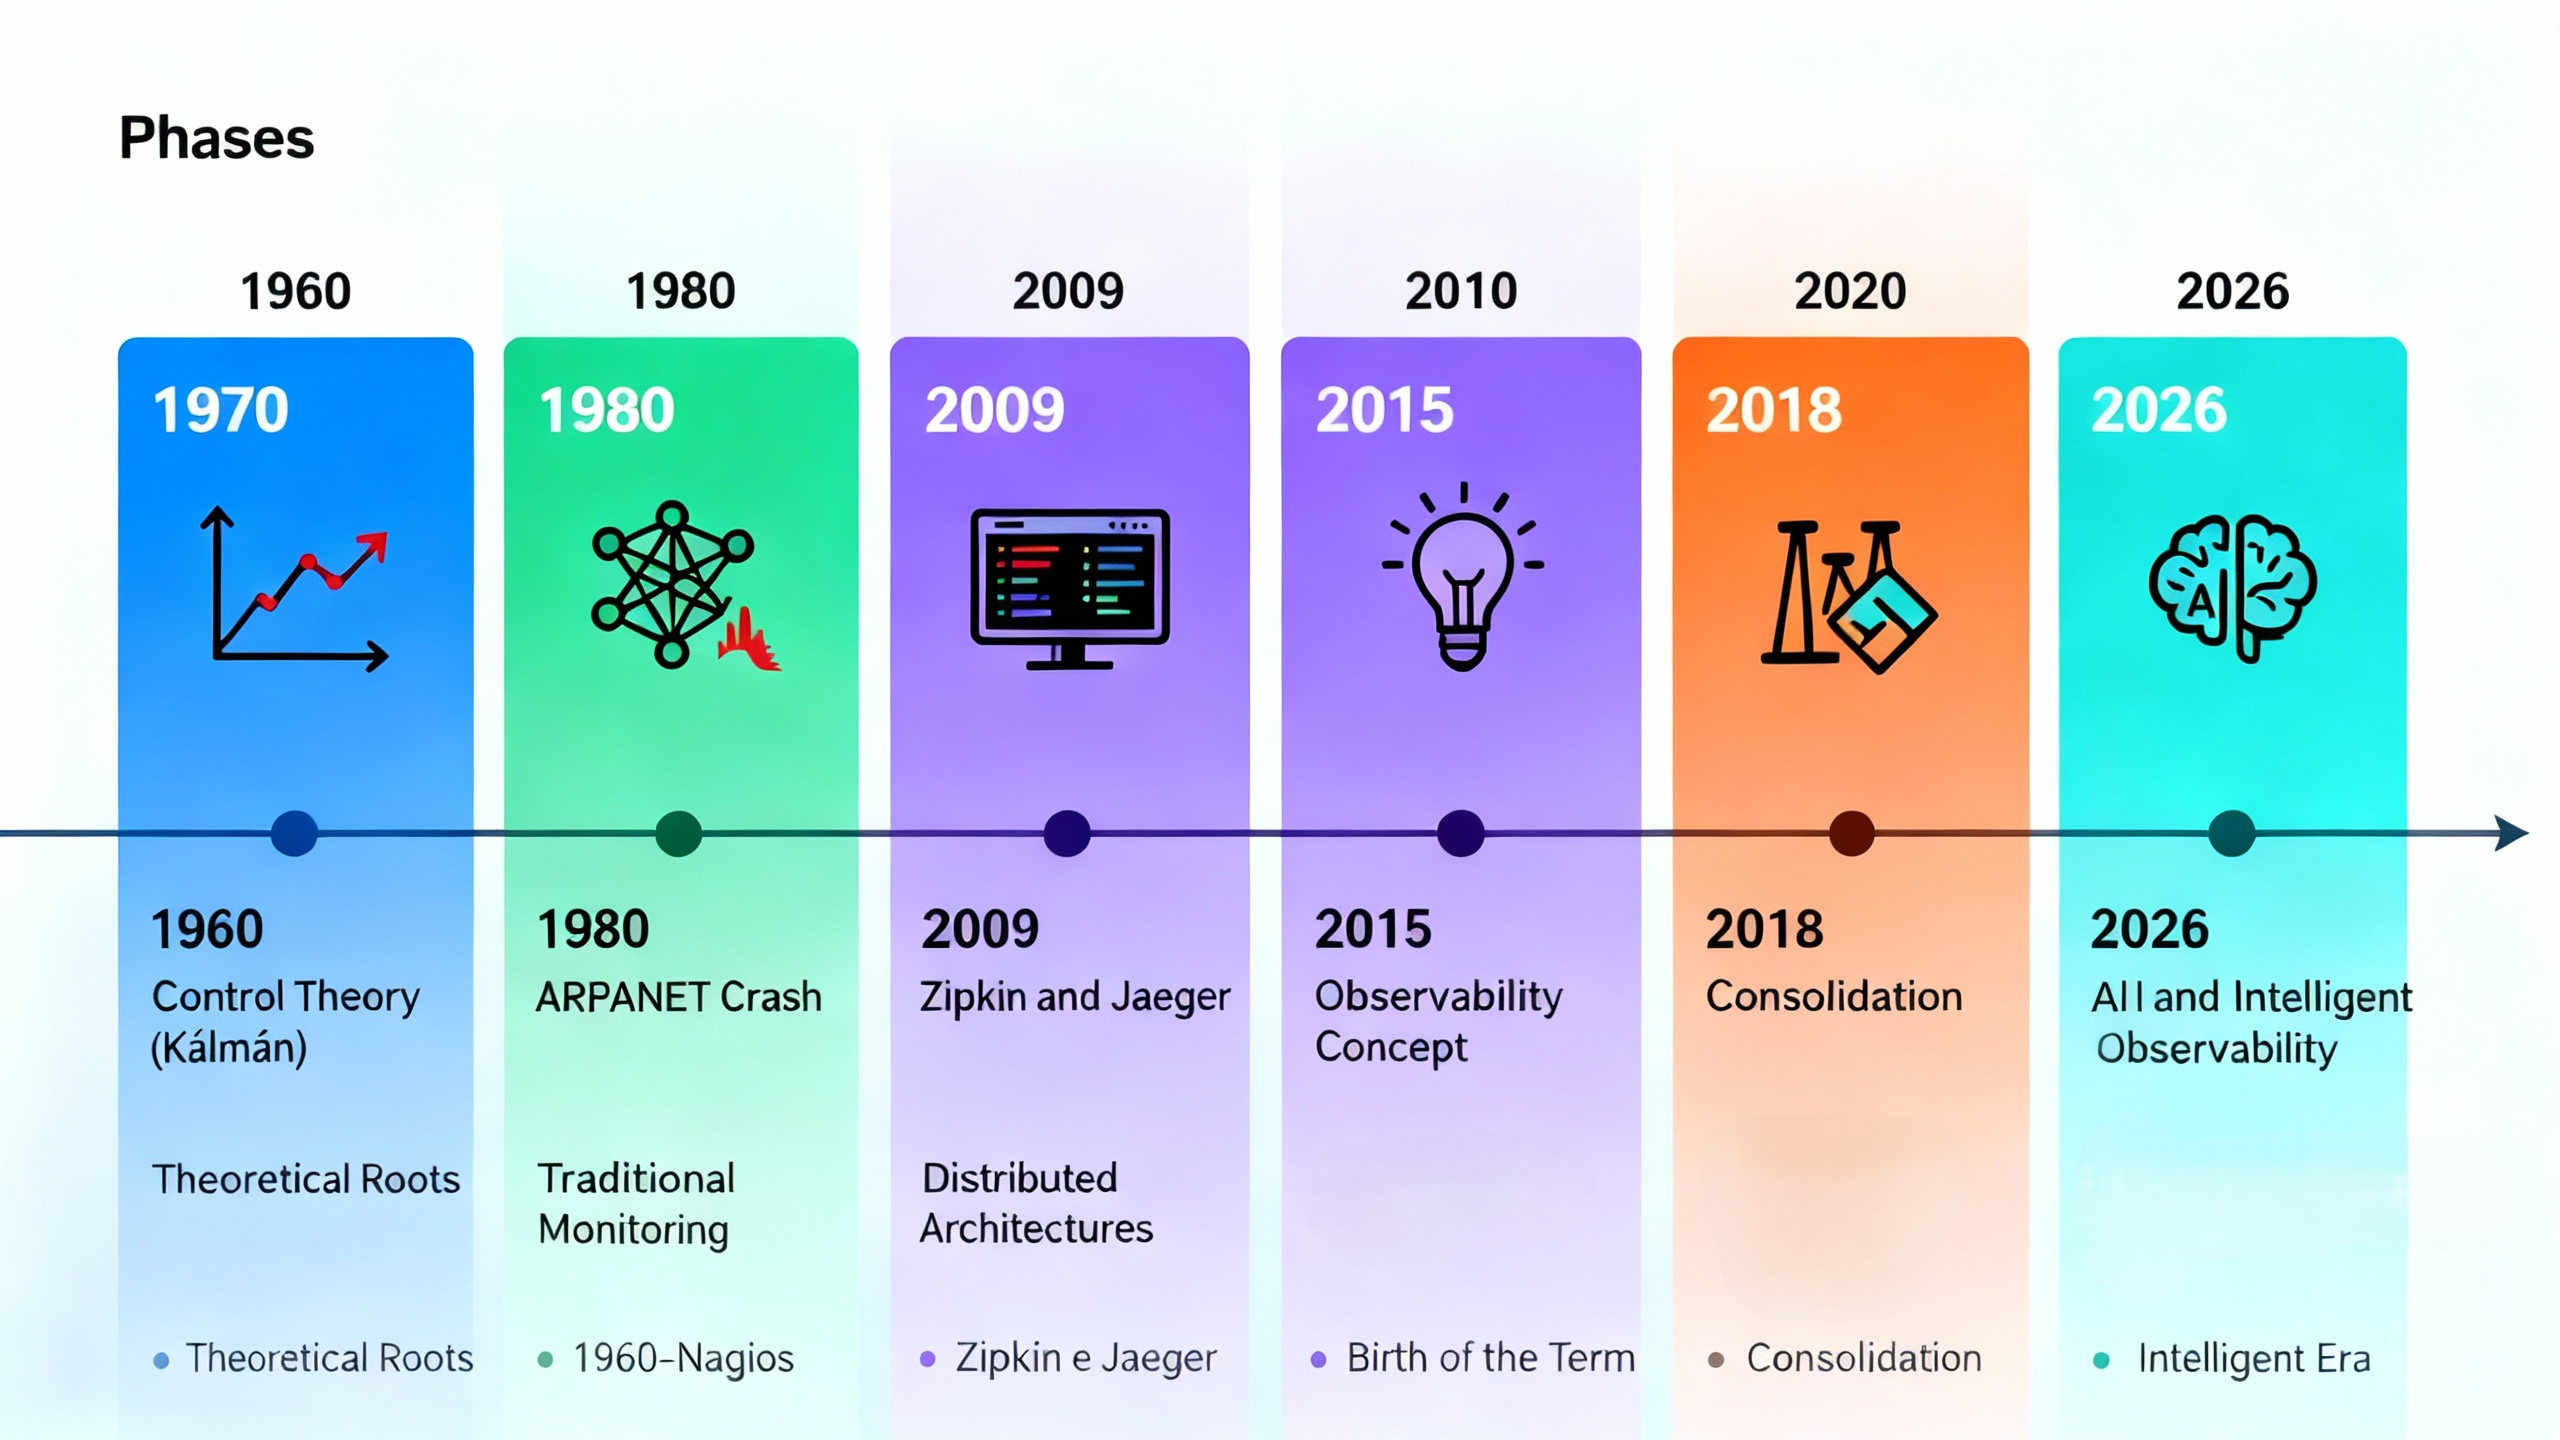
\includegraphics[width=1.0\linewidth]{images/observability/observability-timeline.png}
    \par\medskip\ABNTEXfontereduzida\selectfont\textbf{Source:} Created by author (2026) \par\medskip
\end{figure}

\begin{table}[ht]
\centering
\caption{Evolution of Observability - Comparison Between Historical Phases}
\label{tab:obs-evo}
\resizebox{\textwidth}{!}{%
\begin{tabular}{llllll}
\toprule
\textbf{Period} & \textbf{Paradigm} & \textbf{Architecture} & \textbf{Collected Data} & \textbf{Main Tools} & \textbf{Main Challenge} \\ \midrule
1960-1980 & Control Theory & Monolithic/Centralized & Basic Metrics (CPU, RAM) & Analog Instruments & Limited Visibility \\
1980-2010 & IT Monitoring & Client-Server & Metrics + Simple Logs & Nagios, Zabbix, Cacti & Forecasting Necessary Data \\
2010-2015 & Transition & Early Microservices & Metrics + Logs + Traces & Zipkin, Jaeger, New Relic & Service Correlation \\
2015-2018 & Observability & Distributed Cloud-Native & Logs, Metrics, Traces & Prometheus, Grafana, Loki & Standardization and Scalability \\
2018-2022 & Consolidation & Kubernetes, Serverless & Unified Telemetry & OpenTelemetry, Datadog & Vendor Integration \\
2022-2026 & Intelligence & Distributed + Edge & Telemetry + AI/ML & Cribl, Honeycomb, Datadog & Cost and Complexity \\ \bottomrule
\end{tabular}%
}
  \par\medskip\ABNTEXfontereduzida\selectfont\textbf{Source:} Written by author (2026) \par\medskip
\end{table}

According to \cite{kosinska_2023}, observability in distributed systems is structurally grounded in three foundational telemetry pillars: (i) metrics (collected during continuous runtime activities), (ii) logging, and (iii) distributed tracing. However, as emphasized by \cite{hartikainen_2024}, the mere fact that a system collects these three pillars in isolation does not automatically make it observable; true diagnostic value is obtained only by semantically correlating these pillars and converting them into interpretable state evidence. Furthermore, \cite{bhatia_2025} highlights that modern cloud-native observability frameworks incorporate a fourth essential category: platform events ($O = \{M, L, T, E\}$). Each telemetry modality fulfills a distinct epistemic role in state reconstruction, as synthesized below and illustrated in Figure~\ref{fig:obs-pillars}:

\begin{itemize}
    \item \textbf{Metrics ($M$):} Represent numeric measurements of resource utilization or behavioral rates aggregated over discrete time intervals \cite{ellingwood_2017}. They act as low-overhead counters, gauges, or histograms of system characteristics (e.g., HTTP request throughput, $p95$ response latency, or container CPU and memory saturation).
    \item \textbf{Logs ($L$):} Provide discrete, timestamped records of specific execution events and internal state transitions \cite{beyer_2016}. Logs serve as the primary forensic data source for uncovering the exact error context (e.g., stack traces, connection-reset exceptions, or serialization failures) within an individual process at a given point in time.
    \item \textbf{Distributed Traces ($T$):} Record the causal execution paths taken by requests as they propagate across multi-service architectures \cite{otel_primer_2025, sigelman_2010}. A trace is a directed acyclic graph composed of spans, where each span represents a named, timed unit of work enriched with causal metadata (\texttt{trace\_id}, \texttt{span\_id}, and \texttt{parent\_span\_id}).
    \item \textbf{Events ($E$):} Represent discrete, immutable state-change notifications emitted by the orchestration platform or runtime environment \cite{hartikainen_2024, bhatia_2025}, such as pod scheduling decisions, container OOM terminations, or configuration rollouts.
\end{itemize}

\begin{figure}[ht]
    \centering
    \caption{Observability Pillars}
    \label{fig:obs-pillars}
    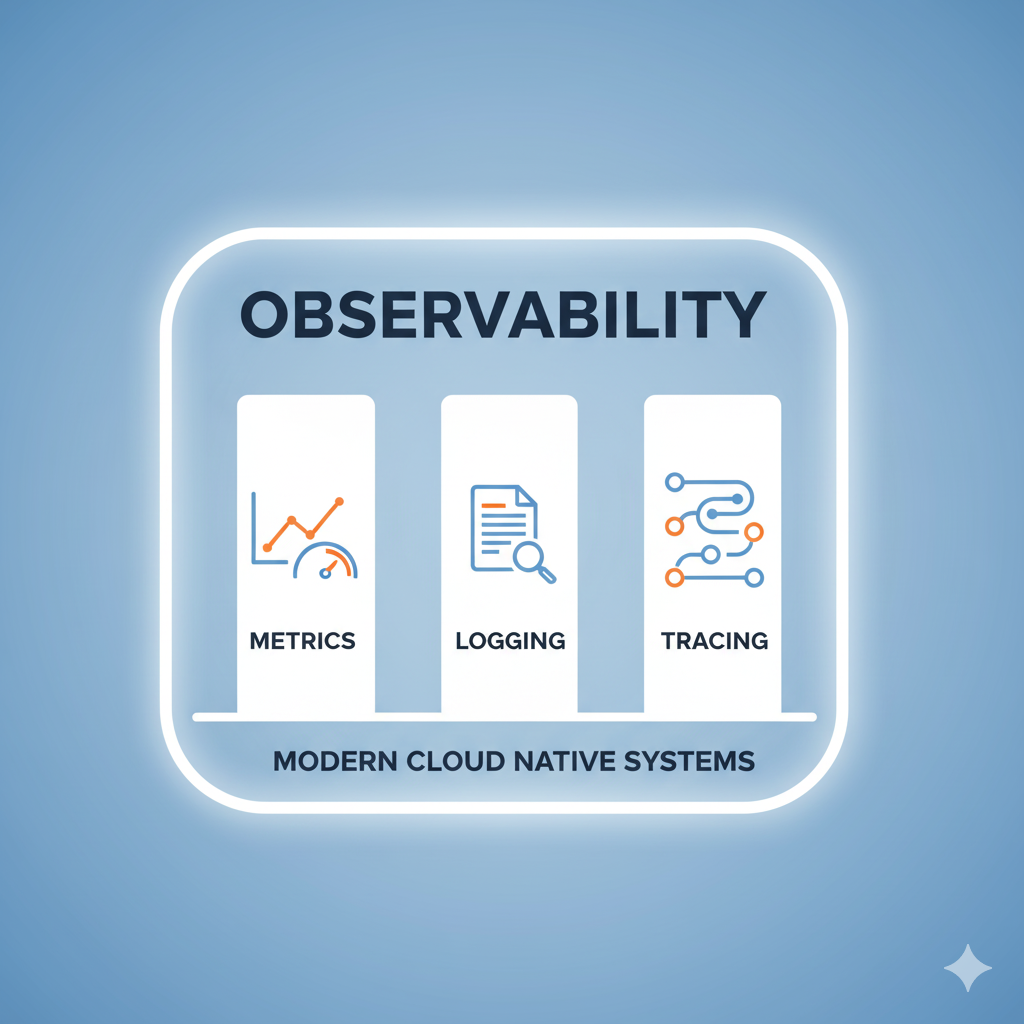
\includegraphics[width=0.75\linewidth]{images/observability/observability-pillars.png}
    \par\medskip\ABNTEXfontereduzida\selectfont\textbf{Source:} Created by author (2026) \par\medskip
\end{figure}

Whenever a complex system needs to be regulated, an instrumentation subsystem must be in place to extract these signals. Formally, an instrument is a mechanism designed to measure a specific physical or computational quantity \cite{ribbens_2013}, while telemetry---derived from the Greek roots \textit{tele} (remote) and \textit{metron} (measure)---is the technology that enables data acquired in one runtime locus to be transmitted and analyzed in another \cite{dondelinger_2013}. In cloud-native environments, the abundance and heterogeneity of telemetry across application, platform, and kernel layers require a fundamental analytical shift beyond conventional monitoring, as examined in the following section.
